\documentclass[12pt]{article}
\usepackage[reqno]{amsmath}
\usepackage{amsfonts}
\usepackage{mathtools}
\usepackage{amssymb}
\usepackage{amsthm}
%\usepackage{multicol}
\usepackage[a4paper, margin=1in]{geometry}
\usepackage{indentfirst}
\usepackage{bm}
\usepackage{hyperref}
\hypersetup{
    colorlinks=true,
    linkcolor=blue,      
    urlcolor=cyan,
}
\renewcommand{\thesection}{\Roman{section}}
\setlength{\parindent}{4em}


\begin{document}
\begin{center}
\par\noindent\rule{\textwidth}{0.6pt}\\[0.3cm]
\textbf{\LARGE{Assignment 2}}\\[0.3cm]
\Large{BT1010 : Introduction to Life Sciences}\\[0.1cm]
\large{April 7, 2021}\\[0cm]
\par\noindent\rule{\textwidth}{0.6pt}
\end{center}
%\begin{multicols}{2}
\noindent
\hspace{0.4cm}Name : Taha Adeel Mohammed
\par \noindent
\hspace{0.4cm}Roll No. : CS20BTECH11052
\section*{Question}
Why are many fossils of marine animals(e.g. ammonites) found in the Himalayas?
\section*{Answer}
%\end{multicols}
More than 150 million years ago, India was part of an immense supercontinent called Gondwana, which included Australia, Africa, Antarctica, India, and South America and covered much of the Southern Hemisphere. Around 120 million years ago, what is now India broke off and started slowly migrating north towards Eurasia. The continent collided with Eurasia about 50 million years ago, giving rise to the Himalayas.
\begin{figure}[h!]
    \centering
      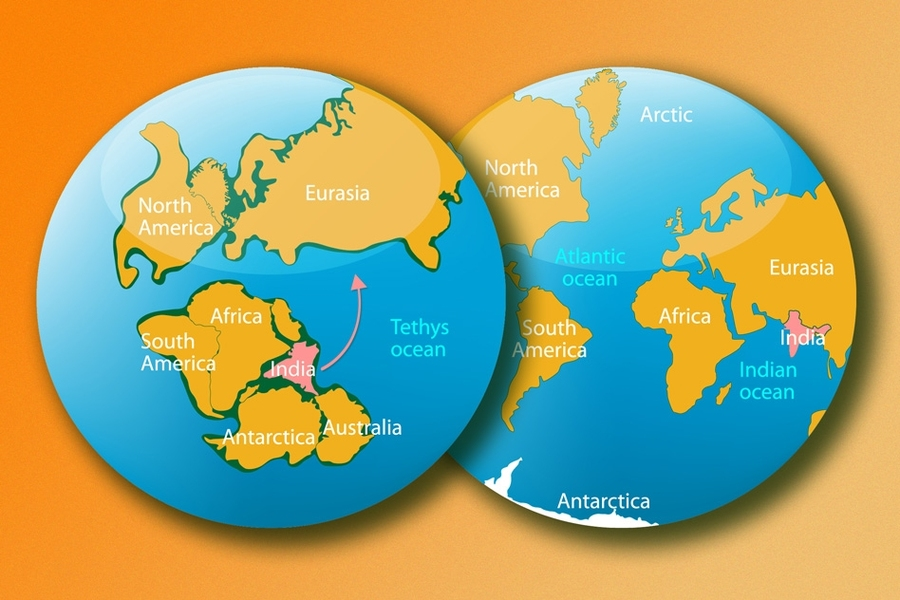
\includegraphics[width=\columnwidth /2]{Figures/MIT-FastDrift_0.jpg}
    \caption{Continental drift of India}\nonumber
\end{figure}
\par The \textbf{Tethys Sea}, which lay between the two land-forms, had a rich and diverse marine life. When they finally collided, it was with so much power that the dense crusts of both, crushed together by the immense force, rose upward, forming mountains that rose from beneath the sea. Hence, fossils of marine creatures that lived millions of years ago that were buried in sedimentary rocks on the ocean floor can be found in the Himalayas.
% build up fat reserves before trying to cross the ocean between Africa and India and secondly to wait for favourable winds which will help them across the waterbody. The falcons will take advantage of strong summer winds, usually the tail-winds from monsoons that occur from May to September. These winds will assist them all the way to the coast of India.\\
%   these Falcons in groups exceeding 30 individuals. \\
%   the greatest over-water crossing of any bird of prey, traversing as much as 2,400 miles of the Indian Ocean. Over water, the hot-air thermals and deflection currents that assist raptors migrating over land, allowing them to soar for hours and save energy, are largely absent. This means the falcons must beat their wings continuously on their transoceanic trip\\
%   Birds going over India are thought to be aided by strong winds blowing westward. These winds are strong at an altitude of about 3000m and the birds are thought to fly at a height of above 1000m during migration\\
%   Their migration over the Arabian Sea coincides with the timing of the migration of dragonflies (Pantala flavescens) and these are thought to provide food during the most arduous part of their migration route.\\
%   Flight 95773(the number given to the Amur falcon bird which is fitted with solar powered transmitter and antenna) Wearing a tiny solar-powered transmitter on her back, and tracked by satellites 850km above, she flies 14 560km, including a 5-daynon-stop journey of 5 912km at 50km/h Satellites track Flight 95773 an Amur Falcon, as she flies to Mongolia from Newcastle (South Africa) with a tiny transmitter on her back. She gives her trackers a showstopper they could never have imagined: a non-stop leg 5 912km over 5 days.\\
%     Her sleek tapered wings power her to speeds of more than 50km/h and allow her to glide on thermals for long distances
\end{document}